\documentclass{standalone}
\usepackage{tikz}
\begin{document}
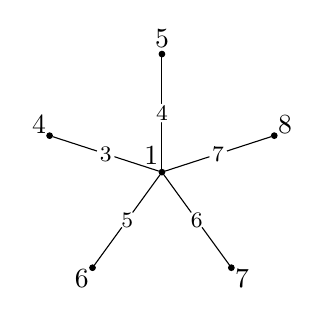
\begin{tikzpicture}[every node/.style={draw, circle, fill=black, minimum size=2pt, inner sep=0pt}]
\node[fill=black, label=above:{$5$}] (G1N1) at (90:1.5) {};
\node[fill=black, label={[yshift=2pt]above left:{$1$}}] (G1N0) at (90:0) {};
\node[fill=black, label=below right:{$7$}] (G1N2) at (306:1.5) {};
\node[fill=black, label=below left:{$6$}] (G1N3) at (234:1.5) {};
\node[fill=black, label=above left:{$4$}] (G1N4) at (162:1.5) {};
\node[fill=black, label=above right:{$8$}] (G1N5) at (18:1.5) {};
\draw (G1N0) -- (G1N1) node (m) [midway, draw =none, fill=white] {\footnotesize$4$}; 
\draw (G1N0) -- (G1N2) node (m) [midway, draw =none, fill=white] {\footnotesize$6$};
\draw (G1N0) -- (G1N3) node (m) [midway, draw =none, fill=white] {\footnotesize$5$} ;
\draw (G1N0) -- (G1N4) node (m) [midway, draw =none, fill=white] {\footnotesize$3$};
\draw (G1N0) -- (G1N5) node (m) [midway, draw =none, fill=white] {\footnotesize$7$};
\end{tikzpicture}
\end{document}
